\chapter{Choosing the Decision Threshold}
\label{ch:p-thresholds}

The common property of scores from the previous lesson is that they depend on the threshold for classifying an instance as positive. We can balance between them by adjusting the threshold to find the required sensitivity at an acceptable specificity. We can even assign costs (monetary or not) to different kinds of mistakes and find the threshold with the minimal expected cost.

A valuable tool to investigate the effects of different thresholds is the Receiver-Operating Characteristic curve. Don’t mind the (historical) meaning of the name and just call it the ROC curve.

Here are the curves for logistic regression, SVM with linear kernels, and naive Bayesian classifier on the same ROC plot.

\begin{marginfigure}
    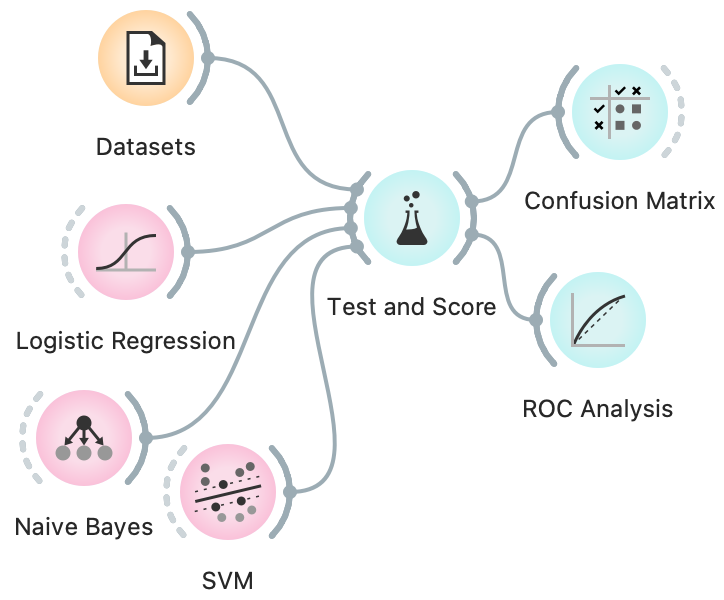
\includegraphics[scale=0.4]{roc-workflow.png}
    \caption{$\;$}
\end{marginfigure}

\begin{figure}[h]
    \centering
    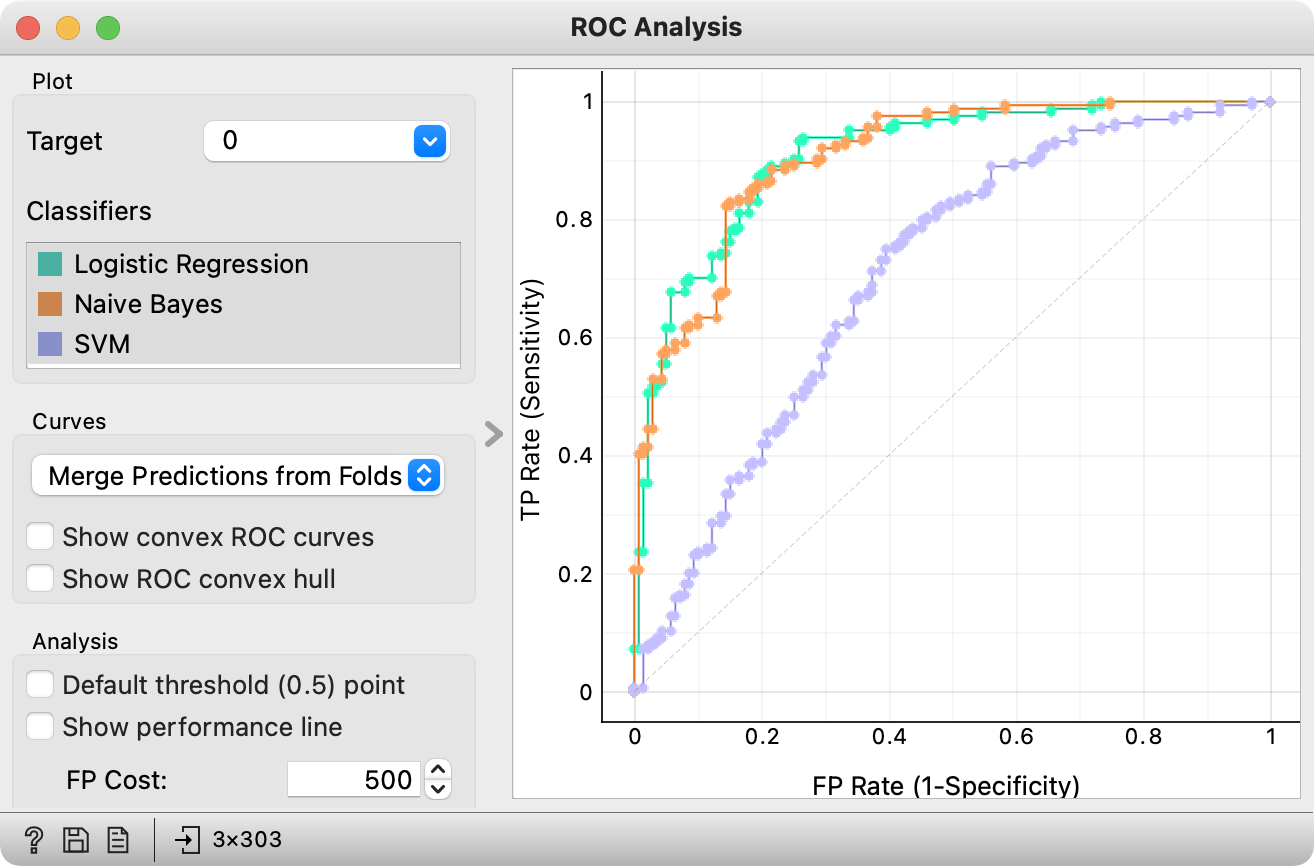
\includegraphics[scale=0.45]{roc-analysis.png}
    \caption{$\;$}
\end{figure}

The curves show how the sensitivity (y-axis) and specificity (x-axis, but from right to left) change with different thresholds.

There exists,\marginnote{\textbf{\textsf{Sounds complicated? If it helps: perhaps you remember the term parametric curve from some of your math classes. ROC is a parametric curve where x and y (the sensitivity and 1 - specificity) are a function of the same parameter, the decision threshold.}}}
for instance, a threshold for logistic regression (the green curve) that gives us 0.65 sensitivity at the specificity of 0.95 (the curve shows 1 - specificity). Or 0.9 sensitivity with a specificity of 0.8. Or a sensitivity of (almost) 1 with a specificity of somewhere around 0.3.

The optimal point would be at the top left. The diagonal represents the behavior of a random guessing classifier.

Which of the three classifiers is the best? It depends on the specificity and sensitivity we want; at some points, we prefer logistic regression and, at other points, the naive bayesian classifier. SVM doesn’t cut it anywhere.

A popular score derived from the ROC curve is called an {\em area under curve}, or AUC for short. It measures, well, the area under the curve. ROC curve. If the curve goes straight up and then right, the area is 1; we can not reach optimal AUC in practice. If the classifier guesses at random, the curve follows the diagonal, and AUC is 0.5. Anything below that is equivalent to guessing or bad luck.

AUC has a kind of absolute scale. As a rule of thumb: 0.6 is bad, 0.7 is bearable, 0.8 is publishable, and anything above 0.95 is suspiciously good.

AUC also has an excellent probabilistic interpretation. Say that we are given two data instances, and we are told that one is positive and the other is negative. We use the classifier to estimate the probabilities of being positive for each instance and decide that the one with the highest probability is positive. It turns out that the probability that such a decision is correct equals the AUC of this classifier. Hence, AUC measures how well the classifier discriminates between the positive and negative instances.

From another perspective: if we use a classifier to rank data instances, then AUC of 1 signifies a perfect ranking, an AUC of 0.5 a random ranking, and an AUC of 0 an ideal reversed ranking.
